\begin{figure}%
	\centering%
	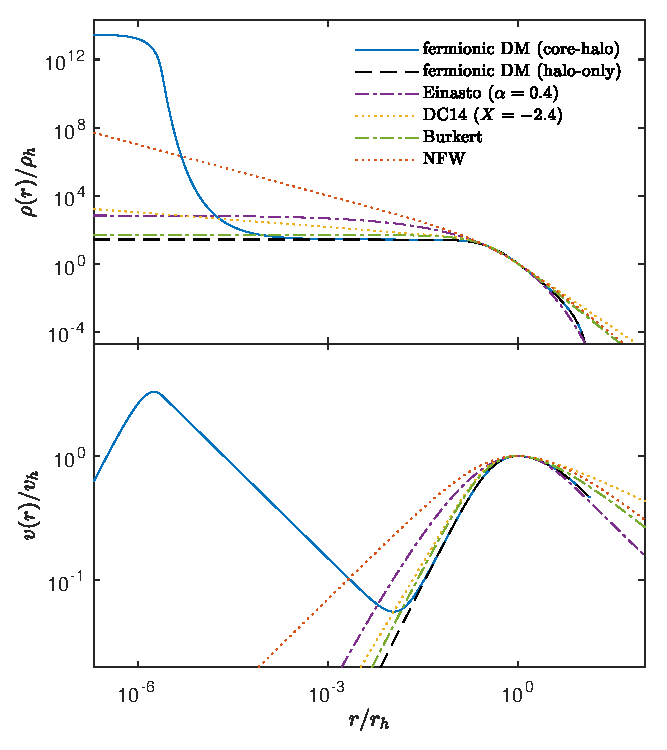
\includegraphics[width=\hsize]{\ROOTPATH/fig.pdf}
	\caption{Rotation curve of NGC0055 with total velocity and baryonic components (bottom). The sum of dark and baryonic components give the total velocities (thick solid lines). The best fitted DM components (top) are given for RAR, NFW and DC14, being compared with the inferred DM from SPARC data. RAR and DC14 produce very similar results despite the underlying physics. NFW is is clearly disfavored here, especially in the inner halo.}%
\label{fig:RC:NGC0055}
\end{figure}